در این فصل به طور اجمالی مروری بر پیش‌زمینه‌ی پژوهش انجام شده است. در هر بخش سعی شده است که با حفظ اختصار، تنها جنبه‌های  کاربردی مرتبط با پژوهش مطرح گردد.
\section{مدل اکتور}
\label{section:actorModel}

در زمینه‌ی برنامه‌نویسی همروند پژوهش‌های مختلفی صورت گرفته و مدل‌هایی ارائه شده است\cite{Briot98concurrencyand}. در این میان مدل \gls{اکتور}\LTRfootnote{Actor Model} با توجه به استفاده از ارتباط ناهمگام و قابلیت توزیع بالا توجه زیادی را به خود جذب کرده است. با توجه به ارتباط تنگاتنگ این مدل با پژوهش حاضر، در این بخش به معرفی اجمالی این مدل می‌پردازیم.
لفظ اکتور برای اولین بار در حدود ۳ دهه پیش توسط هیوئیت  \cite{Hewitt1972} به کار گرفته شد. اکتور در کاربرد هیوئیت به معنی موجودیت‌های فعالی بود که در یک پایگاه دانش به جستجو پرداخته و در نتیجه کنش‌هایی را ایجاد می‌نمودند. در دهه‌های بعدی گروه هیوئیت با تکیه بر اکتورها به عنوان عامل‌های محاسباتی\LTRfootnote{agents of computation} مدل اکتور را به عنوان یک مدل محاسباتی همروند گسترش داد. خلاصه‌ای از تاریخچه‌ی مدل بازیگر در \cite{AghaMST97} موجود است. امروزه برداشت عمومی از مدل اکتور مربوط به  آقا\cite{Agha_86} می‌باشد. در ادامه‌ی این بخش مشخصات مدل اکتور ارائه شده است.
 
مدل اکتور که توسط هیوئیت و آقا \cite{Hewitt1972,Agha1987,Agha1990} ایجاد شده‌است، یک نمایش سطح بالا از سیستم‌های توزیع‌شده فراهم می‌کند. 
\gls{اکتور}هااشیای \gls{لفافه‌بندی‌شده}‌ای هستند که به صورت \gls{همروند} فعالیت می‌کنند و دارای \gls{رفتار}\LTRfootnote{Behavior} قابل تغییر هستند. 
اکتورها \gls{حالت  مشترک}\LTRfootnote{Shared State} ندارند و تنها راه ارتباط بین آنها تبادل ناهمگام پیغام است. 
 در مدل اکتور فرضی در مورد مسیر پیغام و میزان تاخیر در رسیدن پیغام وجود ندارد، در نتیجه ترتیب رسیدن پیغام‌ها \gls{غیرقطعی} است.
 در یک دیدگاه می‌توان اکتور را یک \gls{شی‌ء} در نظر گرفت که به یک ریسمان\gls{ریسمان}\LTRfootnote{Thread} کنترل، یک صندوق پست و یک نام غیر قابل تغییر و به صورت سرارسی یکتا \LTRfootnote{Globally Unique} مجهز شده است. برای ارسال پیغام به یک اکتور، از نام آن استفاده می‌شود. در این مدل، نام  یک اکتور را می‌توان در قالب پیغام  ارسال کرد. پاسخگویی به هر پیام شامل برداشتن آن پیام از صندوق پستی و اجرای عملیات متناسب با آن است.
این اجرای عملیات به صورت \gls{تجزیه‌ناپذیر}\LTRfootnote{Atomic} و بی‌وقفه خواهد بود\cite{Agha_86}.

\begin{figure*}
    \begin{center}
	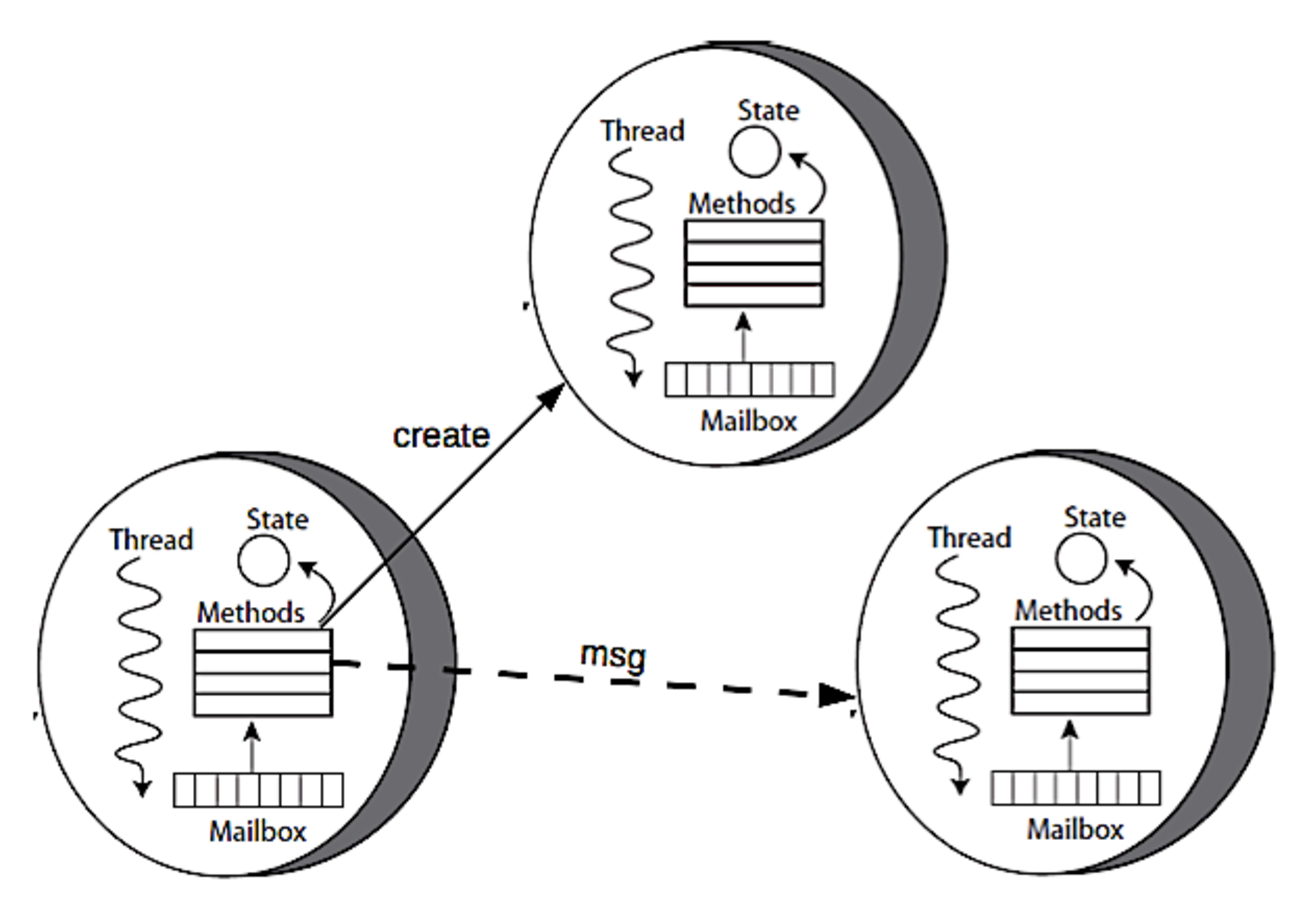
\includegraphics[width=12cm]{2-Preliminaries/Figures/Actor_Structure.pdf}
    \end{center}
    \caption{\label{fig:actorStructure} اکتور‌ها موجودیت‌های همروندی هستند که به صورت ناهمگام تبادل پیغام انجام ‌می‌دهند. }
\end{figure*}


همان گونه که گفته‌شد، مدل اکتور سیستم را در سطح بالایی از انتزاع مدل می‌کند.
این ویژگی دامنهٔ سیستم‌های قابل مدلسازی توسط مدل اکتور را بسیار وسیع نموده‌است.
انواع سیستم‌های سخت‌افزاری و نرم‌افزاری طراحی‌شده برای زیرساخت‌های خاص یا عام، و همچنین الگوریتم‌ها و پروتکل‌های توزیع‌شدهٔ مورد استفاده در شبکه‌های ارتباطی از جملهٔ موارد مناسب برای بهره‌گیری از مدل اکتور هستند. علاوه بر این، خصوصیت تبادل ناهمگام پیغام، باعث می‌شود مدل اکتور برای مدل کردن سیستم‌های توزیع شده و متحرک بسیار ایده‌آل باشد\cite{KarmaniAgha_Actors_11}. شکل \ref{fig:actorStructure} شمای کلی از مدل اکتور و نحوه‌ی تعامل اکتور‌ها را نشان می‌دهد.
 
 یک اکتور در نتیجه‌ی دریافت پیغام احتمالا محاسباتی انجام می‌دهد و در نتیجه‌ی آن یک از ۳ عمل زیر را انجام می‌دهد:
\begin{itemize}
\item ارسال پیغام به سایر اکتور‌ها
\item ایجاد اکتور جدید
\item تغییر حالت محلی
\end{itemize} 

\subsection{\gls{معناشناسی}}\LTRfootnote{Semantics}
از نظر معناشناسی مشخصه‌های کلیدی مدل محض اکتور عبارتند از: لفافه‌بندی و
  \gls{تجزیه‌ناپذیر}‌ی\LTRfootnote{Encapsulation and Atomicity}، \gls{انصاف}\LTRfootnote{Fairness}، 
  استقلال از مکان\LTRfootnote{Location Transparency}، توزیع\LTRfootnote{Distribution} و تحرک\LTRfootnote{Mobility}
 \cite{KarmaniAgha_Actors_11}. 
  باید توجه داشت که این مشخصه‌ها در مدل محض  وجود دارند و این الزاما به این معنی نیست که تمام زبان‌های مبتنی بر مدل اکتور از این مشخصه‌ها پشتیبانی می‌کنند. ممکن است تعدادی از این مشخصه‌ها در  زبان‌های مبتنی بر اکتور  با در نظر گرفتن اهدفی مانند کارایی و سهولت پیاده‌سازی نشده‌اند. در این موارد باید با به کار بردن ابزار‌های بررسی ایستا، مترجم‌ها و یا با تکیه بر عملکرد درست برنامه‌نویس از صحت عملکرد برنامه‌ اطمینان حاصل کرد \cite{ActorsJVM2009}. 
\begin{itemize}
\item \textbf{لفافه‌بندی و \gls{تجزیه‌ناپذیر}ی:}\LTRfootnote{Encapsulation and Atomicity}  
نتیجه‌ی مستقیم مشخصه‌ی لفافه‌بندی در اکتور‌ها این است که درهیچ دو اکتوری، به اشتراک گذاری حالت وجود ندارد. این مشخصه، \gls{تجزیه}ی \gls{شیءگونه}ی برنامه را تسهیل می‌کند. در زبان‌های برنامه‌نویسی \gls{شیء-بنیاد} مشخصه منجر به ایجاد تغییر تجزیه‌ناپذیر شده است. به این صورت که وقتی یک شیء، شیء دیگری را فراخوانی می‌کند، شیء مقصد تا پایان محاسبات مربوط به این فراخوانی، به فراخوانی‌های دیگر پاسخ نمی‌دهد.  این مشخصه به ما اجازه می‌دهد تا بتوانیم در باره‌ی رفتار یک شیء در قبال دریافت یک پیغام (فراخوانی) با توجه به حالت شیء در زمان دریافت آن \gls{استدلال} کنیم.

در محاسبات همروند، وقتی یک اکتور مشغول انجام محاسبات مربوط به یک پیغام است، امکان دریافت پیغام جدید توسط آن وجود دارد اما مشخصه‌ی تجزیه‌ناپذیری تضمین می‌کند که پیغام جدید امکان قطع محاسبات جاری اکتور و تغییر حالت محلی آن را ندارد. این مشخصه الزام می‌کند که اکتور گیرنده، در هر لحظه فقط یک پیغام در حال پردازش داشته باشد و محاسبات مربوط به  پیغام جاری را در یک قدم بزرگ\LTRfootnote{Macro-Step} به صورت تجزیه ناپذیر طی کند. \cite{AghaMST97}
مشخصه‌های معناشناسی لفافه‌بندی و تجزیه ناپذیری به طور  چشم‌گیری از عدم قطعیت مدل اکتور می‌کاهند و با کوچکتر کردن فضای حالت برنامه‌های نوشته شده در مدل اکتور، این برنامه‌ها را برای استفاده در ابزارهای آزمون درستی و  verification(?) قابل استفاده می‌کند\cite{LauterburgKMA10}.
این دو مشخصه مجموعا باعث می‌شوند تا بتوانیم بر اساس پیغام انتخاب شده برای اجرا و وضعیت محلی اکتور در هنگام شروع به اجرا ، رفتار یک اکتور قابل پیش‌بینی باشد.

\item \textbf{ \gls{انصاف}:}
انصاف در مدل اکتور به این مفهوم است که پیغام فرستاده شده نهایتا به اکتور مقصد خواهد رسید، مگر آنکه اکتور مقصد به طور دائمی غیر فعال شده باشد. لازم به ذکر است که این تعریف از  انصاف در رسیدن پیغام به اکتور مقصد، متضمن انصاف در \gls{زمان‌بندی} اکتور‌ها است. به این مفهوم که در صورتی که یک اکتور در اثر  زمان‌بندی غیر منصفانه، موفق به اخذ نوبت اجرا نشود، پیغام‌های فرستاده شده به مقصد آن اکتور هرگز به مقصد نخواهند رسید. انصاف علاوه بر تضمین رسیدن پیغام‌ها، امکان استدلال مناسب درباره‌ی نحوه‌ی تداوم اجرای  برنامه‌\LTRfootnote{Liveness Property} را فراهم می‌کند. میزان طبیعتا میزان موفقیت در تضمین این مشخصه در محیط‌های مبتنی بر اکتور وابسته به منابع موجود در سیستم در حال اجرا است \cite{ActorsJVM2009}.
\item \textbf{ استقلال از مکان، توزیع و تحرک:}
\label{mobility}
در مدل اکتور، ارسال پیغام به یک اکتور تنها از طریق دسترسی به نام آن اکتور ممکن می‌شود. مکان واقعی اکتور تأثیری روی نام آن ندارد. هر اکتور دارای فضای آدرس مربوط به خود است که می‌تواند کاملا متفاوت با دیگر اکتور‌ها باشد. اکتورهایی که به یکدیگر پیغام می‌فرستند می‌توانند روی یک هسته از یک پردازنده‌ی مشترک اجرا شوند یا اینکه در ماشین دیگری که از طریق شبکه به آنها مرتبط می‌شوند در حال اجرا باشند. مشخصه‌ی  استقلال از مکان در مدل اکتور به برنامه‌نویس این امکان را می‌دهد که فارغ از نگرانی درباره‌ی محل اجرای  اکتور ها به برنامه‌نویسی بپردازد.
 عدم اطلاع از مکان اجرای اکتوران  منجر به قابلیت حرکت در آنها می‌شود. تحرک به صورت قابلیت انتقال پردازش به نودهای دیگر تعریف می‌شود.در سطح سیستم، تحرک از جهت توزین بار \LTRfootnote{Load-Balancing}، قابلیت تحمل خطا\LTRfootnote{Fault Tolerance} و نیز پیکربندی مجدد\LTRfootnote{Reconfiguration} حائز 
 اهمیت است.
 پژوهش‌های پیشین نشان می‌دهد که قابلیت تحرک در رسیدن به کارایی \gls{مقیاس‌پذیر} به ویژه در کاربردهای  \gls{بی‌قاعده}\LTRfootnote{Irregular} روی ساختار داده‌های \gls{پراکنده} مفید است\cite{KimA95}. در کاربردهای دیگر، توزیع بهینه به شرایط زمان اجرا و میزان بار وابسته است. به عنوان مثال، در کاربردهای وب، تحرک با توجه به شرایط شبکه و امکانات کلاینت مورد استفاده قرار می‌گیرد\cite{ContextAwareWeb}.  
از سوی دیگر، قابلیت تحرک می‌تواند در کاهش انرژی مصرفی در اثر اجرای کاربردهای موازی مفید باشد. در این کاربردها، محاسبات موازی به صورت پویا بین تعداد هسته‌های بهینه (تعداد هسته‌هایی که منجر به کمترین مصرف می‌شوند) توزین می‌شوند. قسمت‌های مختلف یک کاربرد می‌تواند شامل الگوریتم‌های موازی مختلفی باشد و میزان مصرف انرژی یک الگوریتم به تعداد هسته‌های مشغول اجرای الگوریتم و نیز بسامد اجرای آن هسته‌ها بستگی دارد\cite{KorthikantiA10}. در نتیجه، ویژگی تحرک پذیری اکتور‌ها، ویژگی مهمی برای برنامه نویسی در معماری‌های چند-هسته‌ای به شمار می‌آید.

\end{itemize} 


\subsection{پیاده‌سازی‌ها}
\label{subsection:actorImpls}
برای مدل اکتور زبان‌ها و چارچوب‌های زیادی توسعه داده شده است. ABCL، POOL، ConcurrentSmalltalk، ACT++ و CEiffel تعدادی از پیاده‌سازی‌های اولیه از این مدل می‌باشند. مرجع \cite{Briot98concurrencyand} به بررسی این زبان‌ها پرداخته است. شاید بتوان زبان  \gls{ارلانگ}\LTRfootnote{Erlang}\cite{erlang} را معروفترین پیاده‌سازی مدل اکتور دانست. این زبان در حدود ۲۲ سال قبل برای برنامه‌نویسی سوئیچ‌های مخابراتی شرکت اریکسون\LTRfootnote{Ericsson} توسعه داده شد. علاوه بر ارلانگ زبان‌ها و چارچوب‌های مبتنی بر مدل اکتور دیگری نیز در سال‌های اخیر مورد استفاده گرفته‌اند که کتابخانه‌ی اکتور اسکالا
\LTRfootnote{Scala Actor Library} \cite{ScalaActors}،  Ptolemy \cite{Ptolemy}، SALSA \cite{salsa}، CHARM++ \cite{CHARMplus}، ActorFoundry \cite{ActorFoundry}، Asynchronous Agents Library \cite{AsyncAgentsLib}  از جمله‌ی آنها هستند.
  از کاربردهای متن-باز که بر مبنای مدل اکتور توسعه داده شده‌اند می‌توان به سیستم تبادل پیغام توئیتر\LTRfootnote{Twitter} و چارچوب تحت وب لیفت\LTRfootnote{Lift} و از میان کاربرد‌های تجاری می‌توان به سیستم گپ\LTRfootnote{Chat} فیسبوک و موتور بازی وندتا\LTRfootnote{Vendetta game engine} اشاره کرد.
در این پژوهش برای پیاده‌سازی نسخه‌ی مبتنی بر تبادل ناهمگام پیغام از کتابخانه‌ی اکتور اسکالا استفاده شده است (چرا؟) که در بخش ؟ معرفی شده است.


\section{معرفی زبان اسکالا و کتابخانه‌ی اکتور اسکالا}
\label{section:Scala}
همان طور که در بخش \ref{subsection:actorImpls} اشاره شد، پیاده‌سازی‌های مختلفی از مدل اکتور در زبان‌ها و چارچوب‌های برنامه‌نویسی ارائه شده است. مقاله‌ی \cite{ActorsJVM2009} به بررسی و مقایسه‌ی این پیاده‌سازی‌ها پرداخته است. در این پژوهش زبان اسکالا و کتابخانه‌ی اکتور آن برای پیاده‌سازی مطالعه‌ی موردی انتخاب شده است. گستردگی ابزار و همچنین فعال بودن جامعه\LTRfootnote{Community}‌ی برنامه‌نویسی این زبان اصلی‌ترین انگیزه‌های انتخاب این زبان برای پیاده‌سازی بوده‌اند. ضمنا با توجه به انتخاب زبان جاوا برای پیاده‌سازی نسخه‌ی متداول مورد مطالعه و ارتباط تنگاتنگ زبانهای اسکالا و جاوا، انتخاب زبان اسکالا منجر به سهولت ارزیابی مقایسه‌ای مطالعه‌ی موردی شده است. در این بخش به معرفی اجمالی زبان اسکالا و کتابخانه‌ی اکتور آن پرداخته شده است. هدف از این معرفی، سهولت درک روش طراحی پیشنهادی در فصل ۳ می باشد و به همین دلیل از توضیح جزئیات و امکانات اضافی این زبان خودداری شده است. کتاب \cite{programmingInScala} به عنوان منبع اصلی این بخش استفاده شده است.
\subsection{زبان اسکالا}
اسکالا مخفف عبارت \emph{''زبان مقیاس‌پذیر``}\LTRfootnote{Scalable Language} است و اشاره به این نکته دارد که اسکالا برای رشد بر اساس نیاز کاربر طراحی شده است. اسکالا را می‌توان برای گستره‌ی وسیعی از کاربردها از نوشتن اسکریپت‌های کوچک گرفته تا پیاده‌سازی سیستم‌های بزرگ به کار برد. برنامه‌های اسکالا بر روی محیط اجرایی جاوا\LTRfootnote{JRE}  قابل اجرا هستند و در برنامه‌های اسکالا  می‌توان از کتابخانه‌های استاندارد جاوا استفاده کرد.
زبان اسکالا ترکیبی از ویژگی‌های زبان‌های \gls{تابعی} و شیءگرا را در خود دارد. در زبان‌های تابعی، توابع مانند انواع داده‌ها قابل ارجاع هستند. اسکالا مانند جاوا دارای \gls{بررسی گونه‌ها}ی، \gls{ایستا} است.
\codelisting[language=scala]{2-Preliminaries/src/Sample.scala}{قطعه کد نمونه برای زبان اسکالا}{figure:scalaSample}

در ادامه مشخصات نحوی زبان اسکالا در قالب یک مثال توضیح داده می‌شود. در شکل \ref{figure:scalaSample} قطعه کد اسکالا مربوط به کلاس Course نمایش داده شده است. برای آشنایی با نحو زبان اسکالا به بررسی این کد می‌پردازیم:\\
در خطوط ۱و ۲ کلاس Course و متغیرهای ،id ،name units و prerequisites به عنوان فیلد‌های آن تعریف شده‌اند. در خط ۴ تابع equals از این کلاس override شده است. در اسکالا همانند جاوا هر کلاس به طور پیش‌فرض دارای یک تابع‌ equals است که در صورت لزوم می‌توان آن را override کرد. همان‌طور که در کد مشخص است، تعریف تابع در اسکالا با کلمه‌ی کلیدی  \textbf{def} انجام می‌گیرد. در خطوط ۴ تا ۸ شرط لازم برای یکسان بودن یک شیء از نوع Course با شیء حاضر پیاده‌سازی شده است. نوع و مقدار یک متغیر را می‌توان با استفاده از دستور \lr{match .. case .. } با انواع و مقادیر دلخواه مقایسه کرد. نتیجه‌ی دستورات خطوط ۶ و ۷ این است که اگر متغیر other از نوع Course باشد و مقدار فیلد id آن با مقدار فیلد id از شیء حاضر یکسان باشد تابع مقدار true را برمی‌گرداند. خط ۸ به این معنا است که اگر هر حالت دیگری به جز حالت قبل بود مقدار false برگردانده ‌می‌شود. در خط ۱۲ ‌نمونه‌ای از حلقه‌ی for نمایش داده شده است. در اسکالا حلقه‌ها به صورت‌های متنوعی می‌توانند بیان شوند که در این مثال یک حالت از آنها نمایش داده شده است.  در خط ۱۲ متغیر pre برای گرفتن مقدار موقت حلقه تعریف شده است. نکته‌ی جالب توجه این است که در این خط، نوع متغیر تعریف نشده است. در بخش قبل ذکر شد که اسکالا دارای خاصیت بررسی گونه‌های ایستا \LTRfootnote{static type checking} است. ظاهرا این دو امر در تناقض با یکدیگر هستند اما باید توجه داشت که در زبان اسکالا نوعی از استنتاجِ گونه\LTRfootnote{type inference} در زمان ترجمه اتفاق می‌افتد. در این مورد با توجه به اینکه متغیر pre از لیست prerequisites مقداردهی می‌شود، گونه‌ی آن در زمان ترجمه قابل استنتاج است. خط ۱۶ تابع دیگری را نشان می‌دهد که در آن تابع toString، override شده است. نکته‌ی قابل توجه در مورد این قسمت از کد عدم استفاده از علامت \{ \} برای تعیین حوزه‌ی تابع است. در زبان اسکالا به دلیل وجود ویژگی‌های زبان‌های تابعی، می‌توانیم با توابع مانند متغیر‌ها و داده‌ها رفتار کنیم که این بخش از کد مثالی از این ویژگی است. همانطور که در این مثال مشخص است، در زبان اسکالا استفاده از نقطه‌ویرگول (;) در اکثر موارد اختیاری است.

\subsection{کتابخانه‌ی اکتور اسکالا}
\label{section:scalaActorLib}
همانطور که در بخش \ref{subsection:actorImpls} اشاره شد، یکی از پیاده‌سازی‌های مدل اکتور، کتابخانه‌ی اکتور اسکالا است. در این بخش به معرفی اجمالی کتابخانه‌ی اکتور اسکالا و طرز استفاده از آن برای برنامه‌نویسی همروند می‌پردازیم.
\subsubsection{ایجاد اکتور}
اکتور‌ها در اسکالا از کلاس scala.actors.Actor مشتق می‌شوند.  شکل \ref{figure:sillyActor} کد مربوط به  یک اکتور ساده را نشان می‌دهد. این اکتور کاری به صندوق پیغام‌ها ندارد و صرفا پنج بار پیغام \lr{I'm acting!} را چاپ می‌کند و سپس اجرای آن خاتمه می‌یابد.

\codelisting[language=scala]{2-Preliminaries/src/SillyActor.scala}{کد یک اکتور ساده در زبان اسکالا}{figure:sillyActor}

  اکتور‌ها در اسکالا با دستور start() شروع به فعالیت می‌کنند. با شروع به فعالیت یک اکتور، تابع act() آن فراخوانی می‌شود و تا زمانی که اجرای این تابع به اتمام نرسد، اکتور به طور همروند در حال اجرا باقی می‌ماند. در صورتی که بخواهیم اکتور به طور دائمی در حال اجرا بماند دو راه وجود دارد. راه اول این است که تابع act() را در پایان کار  خود مجدداً فراخوانی کنیم. و راه دیگر استفاده از عبارت \textbf{loop} در اسکالا است. دستورات درون حلقه‌ی loop به صورت بی‌پایان اجرا می‌شوند. شکل \ref{fig:endlessActor} کدهای مربوط به این ۲ روش را نمایش می‌دهد.

\begin{figure*}
    \begin{center}
    \begin{tabular}{ c  c }
      	%\hline
	 & \\

	\begin{latin}
\linespread{1.1}
\lstinputlisting[language=scala]{2-Preliminaries/src/SillyActor2.scala}
\end{latin} & 
 \begin{latin}
	\linespread{1.1}
	\lstinputlisting[language=scala]{2-Preliminaries/src/SillyActor3.scala}
\end{latin}
 	\\
         (الف) & (ب) \\
%	\hline
    \end{tabular}
    \end{center}
    \caption{\label{fig:endlessActor} تداوم اجرای اکتور با استفاده از الف)فراخوانی بازگشتی و ب)حلقه‌ی loop}
\end{figure*}


\subsubsection{تبادل پیغام}
عملگر \textbf{!} برای فرستادن پیغام ناهمگام استفاده می‌شود. دستور \lr{dest ! message} پیغام message را برای اکتور dest ارسال می‌کند بدون آنکه برای دریافت جواب منتظر بماند. با اینکه در مدل اکتور دستوری برای تبادل همگام پیغام وجود ندارد، در اکثر پیاده‌سازی‌ها این امکان به مدل اضافه شده است\cite{ActorsJVM2009}. در کتابخانه‌ی اکتور اسکالا، عملگر \lr{!?} به این منظور به کار گرفته می‌شود. در صورت استفاده از این دستور، فرستنده‌ی پیغام بلافاصله بعد از ارسال پیغام، تا گرفتن پاسخ متوقف می‌ماند. عملگر دیگری که برای تبادل پیغام مورد استفاده قرار می‌گیرد \lr{!!} است. این عملگر که در کتابخانه‌ی اسکالا به عنوان \gls{آینده}\LTRfootnote{Future} شناخته می‌شود، برای حالاتی به کار می‌رود که دریافت پاسخ را می‌توان به صورت محدود به آینده مؤکول کرد. خروجی این عملگر آرایه‌ای است که هر عضو آن یک تابع است. با فراخوانی هر تابع، اکتور تا دریافت پاسخ متناظر متوقف می‌شود.
%TODO ADD EXAMPLES HERE
برای برداشتن پیغام از صندوق پیغام‌ها، از دو دستور receive و react استفاده می‌شود (تفاوت این دو دستور در بخش \ref{ref:receive_react} توضیح داده شده است). شکل \ref{fig:pingPongActor} مثالی از نحوه‌ی تبادل پیغام بین اکتوران را نمایش می‌دهد. در این برنامه دو اکتور PingActor و PongActor به تبادل پیغام می‌پردازند. در ابتدا اکتور PingActor که متغیر آن با مقدار ۱۰۰ مقداردهی شده است یک پیغام Ping برای اکتور PongActor می‌فرستد و در ادامه در یک حلقه‌ی loop منتظر پاسخ Pong می‌ماند. اکتور PongActor با گرفتن هر پیغام Ping پاسخ Pong را برای فرستنده ارسال می‌کند. کلمه‌ی کلیدی \textbf{sender} در کلاس Actor اشاره‌گری به فرستنده‌ی پیغام در حال پردازش ‌می‌باشد (خط ۶ از کد قسمت (ب) شکل \ref{fig:pingPongActor}). اکتور PingActor با دریافت پاسخ‌ Pong مقدار متغیر pingsLeft را چک می‌کند و در صورت مثبت بودن آن پیغام Ping بعدی را ارسال می‌کند و در غیر این صورت پیغام Stop را ارسال ‌می‌کند. نهایتا با صفر شدن متغیر pingsLeft، اکتور PingActor پیغام Stop را برای PongActor می‌فرستد. دستور exit که در پایان کار هر دو اکتور استفاده شده است باعث می‌شود ریسمان اجرایی اکتور رها شود و پس از اجرای این دستور اکتور قادر به دریافت پیغام نخواهد بود.

\begin{figure*}
    \begin{center}
    \begin{tabular}{ c }
 \begin{latin}
	\linespread{1.1}
	\lstinputlisting[language=scala]{2-Preliminaries/src/Ping.scala}
\end{latin}
\\ 
\scriptsize{(الف) اکتور Ping که فرستنده‌ی اولیه‌ی پیغام است}
&
\hline
\\
\begin{latin}
\linespread{1.1}
\lstinputlisting[language=scala]{2-Preliminaries/src/Pong.scala}
\end{latin}  
\\
\scriptsize{(ب) اکتور Pong که به پیغام ping پاسخ می‌دهد.}
          &
\hline
\begin{latin}
\linespread{1.1}
\lstinputlisting[language=scala]{2-Preliminaries/src/PingPong.scala}
\end{latin} 
\\
\scriptsize{(ج) کد اجرای برنامه‌ی PingPong}
         &
\hline

\end{tabular}
\end{center}
\caption{\label{fig:pingPongActor} مثالی از نحوه‌ی تبادل پیغام بین اکتور‌ها}
\end{figure*}

\subsubsection{ زیرساخت اجرای همروند در کتابخانه‌ی اکتور اسکالا}
\label{ref:receive_react}
پردازش‌های همروند مانند اکتور‌ها با دو نوع استراتژی پیاده‌سازی می‌شوند:
\begin{itemize}
\item \textbf{پیاده‌سازی \gls{ریسمان-بنیان}:}
در این نوع پیاده‌سازی رفتار پردازش همروند به وسیله‌ی یک ریسمان کنترل می‌شود. حالت اجرا\LTRfootnote{execution state} به وسیله‌ی  \gls{پشته}‌ی ریسمان\cite{concurrent_prog_java}

\item \textbf{پیاده‌سازی \gls{رویداد-بنیان}:}
در این مدل رفتار به کمک یک سری \gls{مجری رویداد}\LTRfootnote{event handler} پیاده‌سازی می‌شوند. این مجری‌ها از یک حلقه‌ی رویداد فراخوانی می‌شوند. حالت اجرای پردازش‌های همروند در این روش به کمک رکورد‌ها یا اشیاء مشخصی که به همین منظور طراحی شده‌اند نگهداری می‌شود \cite{SEDA}.
\end{itemize}
مدل ریسمان-بنیان معمولا پیاده‌سازی راحتتری دارد ولی به دلیل مصرف حافظه‌ی بالا و پرهزینه بودن \gls{تعویض متن}\LTRfootnote{context switch} می‌تواند منجر به کارایی کمتری شود\cite{WhyThreadsAreABadIdea}. از طرف دیگر مدل رویداد-بنیان معمولا کاراتر است ولی در طراحی‌های بزرگ پیاده‌سازی آن مشکل‌تر است\cite{whyevents}.
استفاده از مدل رویداد-بنیان منجر به ایجاد نوعی از \gls{وارونگی کنترل}\LTRfootnote{Inversion of Control} می‌شود: یک برنامه به جای فراخوانی عملیات \gls{مسدود کننده} \LTRfootnote{blocking operation}، صرفا تمایل خود به ادامه‌ی کار در صورت رخ دادن رویدادهای مشخص (مانند فشردن یک دکمه) را به محیط اجرا اعلام می‌کند. این اعلام تمایل با ثبت یک مجری رویداد در محیط انجام می‌شود. برنامه هیچ وقت این مجری‌های رویداد را فراخوانی نمی‌کند بلکه محیط اجرایی با وقوع هر رخداد، مجری‌های ثبت شده برای آن رویداد را فراخوانی می‌کند. به این ترتیب کنترل اجرای منطق برنامه نسبت به حالت بدون رویداد \textbf{وارونه} می‌شود. به دلیل پدیده‌ی وارونگی کنترل، تبدیل یک مدل ریسمان-بنیان به مدل رویداد-بنیان معادل معمولا نیاز به دوباره‌نویسی برنامه دارد\cite{responders2006}.
\\
در پیاده‌سازی زیرساخت همروندی در کتابخانه‌ی اکتور اسکالا هر دو رویکرد معرفی شده پیاده‌سازی شده‌اند و قابل دسترسی هستند. اصلی‌ترین عمیات مسدود کننده در مدل اکتور انتظار برای دریافت پیغام است. کنترل اجرا در صورتی مسدود می‌شود که پیغامی که اکتور منتظر دریافت آن است در صندوق پیغام موجود نباشد. در اکتور‌های اسکالا، عمل برداشتن پیغام با دو دستور انجام می‌شود:
\begin{itemize}
\item دستور receive:
با استفاده از این دستور، در صورتی که در صندوق پیغام اکتور، پیغامی که با یکی از الگوهای معرفی شده در بدنه‌ی receive موجود باشد کد مربوط به الگوی‌ مربوطه اجرا می‌شود. در غیر این صورت ریسمان اجرای این اکتور مسدود می‌شود. در این حالت پشته‌ی فراخوانی تابع act() در اکتور به صورت خودکار توسط محیط اجرایی ذخیره می‌شود و در صورت ورود پیغام متناسب اجرا به صورت ترتیبی از سر گرفته می‌شود. بنابراین در پیاده‌سازی این دستور از رویکرد ریسمان-بنیان استفاده شده است.
\item دستور react:
با استفاده از این دستور، در صورتی که هیچ پیغام متناسبی در صندوق پیغام وجود نداشته باشد، به جای مسدود کردن ریسمان اجرای اکتور، از رویکرد رویداد-بنیان استفاده می‌شود. این کار از طریق نوع خاصی از تابع در زبان اسکالا انجام می‌شود که هیچ‌گاه به طور معمولی اجرای آن خاتمه نمی‌یابد. بلکه پس از ثبت مجری رویداد مناسب در محیط اجرا، با استفاده از ایجاد یک \gls{استثناء}\LTRfootnote{exception} اجرای تابع react و توابع شامل آن در اکتور خاتمه می‌یابد. در این نوع توقف اجرا با توجه به اینکه ریسمان اجرا مسدود نمی‌شود، پشته‌ی فراخوانی تابع نیز ذخیره نمی‌شود و با برگشت به اجرای این تابع، محیط هیچ تاریخچه‌ای از اجرای قبلی آن ندارد. در نتیجه در هر بار بازگشت مانند اولین اجرا رفتار می‌کند. نتیجه‌ی مهم این خصوصیت این است که در صورت استفاده از react در یک اکتور، هیچ کدی که بعد از این تابع نوشته شده باشد اجرا نخواهد شد. به همین دلیل برنامه‌نویس باید دقت کند که تابع react از نظر ترتیب اجرا همیشه آخرین کد بدنه‌ی یک اکتور باشد.
نتیجه‌ی استفاده از رویکرد رویداد-بنیان در اکتور‌های اسکالا افزایش چشمگیر کارایی در صورت استفاده از تعداد بسیار زیاد اکتور در سیستم است. 
\end{itemize}
به برنامه نویسان توصیه شده است که به جز در موارد خاص که نیاز به مسدود کردن ریسمان اجرای اکتور وجود دارد، در بقیه‌ی موارد از رویکرد رویداد-بنیان استفاده کنند. توضیحات تکمیلی در مورد نحوه‌ی پیاده‌سازی هر دو رویکرد در کتابخانه‌ی اکتور اسکالا و آنالیز کارایی و مقایسه با سایر پیاده‌سازی‌های مدل اکتور در  \cite{Haller2009202} قابل دسترس می‌باشد.

